%%%%% fs-run-time-impl   Implementation

\label  {fs-implementation-section}

\subsection{Grouping semantics}
The grouping operation was defined in the previous section. Particularly, we assumed that data items get in grouping in the order, provided by the global time. However, this restriction is hard to satisfy in our model, because it supports cycles. Therefore, our implementation of grouping satisfies two conditions:

\begin{enumerate}
\item All correct tuples are eventually produced.
\item Only a limited number of invalid tuples can be generated.
\end{enumerate}

The correctness of tuple means that this tuple would be generated if the order assumption was satisfied. 

As it was mentioned, grouping stores all input items in buckets by the value of hash function. Since the order of input items is arbitrary, we can only maintain the order of items within buckets. Hence, our implementation of grouping semantics includes two steps, which are detailed in the next two subsections. The way to prevent outputting wrong tuples from sink is described further.

\subsubsection{Invalidation}
Our implementation of grouping semantics requires replaying of tuples, which is described in details in the next subsection. However, now, we should notice that replaying can generate tuples with the same global time. Because of the cycles, such items can get in grouping. Therefore, there is a need to remove them from the buckets, because they can produce an unbounded number of invalid tuples. To achieve this goal we introduce the invalidation relation between two data items. Therefore, if new item {\it B} invalidates item {\it A}, item {\it B} replaces item {\it A} in the bucket.

The data item {\it A} is said to be invalidated by the data item {\it B} if:
\begin{enumerate}
\item They have the same global time
\item The trace of {\it A} is less than the trace of {\it B}
\item The first difference is in logical time
\end{enumerate}
If the first difference is in child id, i.e. the items are brothers, there is no invalidation relation between them. Hence, the invalidation relation is a partial order.

Notably, the invalidation relation cannot be lost, when item is go through other operations, because the trace of local times is append-only. This property is applied further, to invalidate items before they get in sink.

\subsubsection{Replaying}

The replaying is used to eventually produce all correct tuples. If the item is get in grouping, according to the global time order, nothing is replayed. If the item is out-of-order and/or it invalidates other item, then all tuples, which contain this element, are reproduced. The example of invalidation and replaying is shown on the figure~\ref{grouping-invalidation-figure}. In this example, the green item is out-of-order and, moreover, it invalidates red item.

Thereby, replaying guarantees that eventually all correct tuples are produced. At the same time, invalidation prevents from producing the unbounded number of incorrect tuples. 

\begin{figure}[htbp]
  \centering
  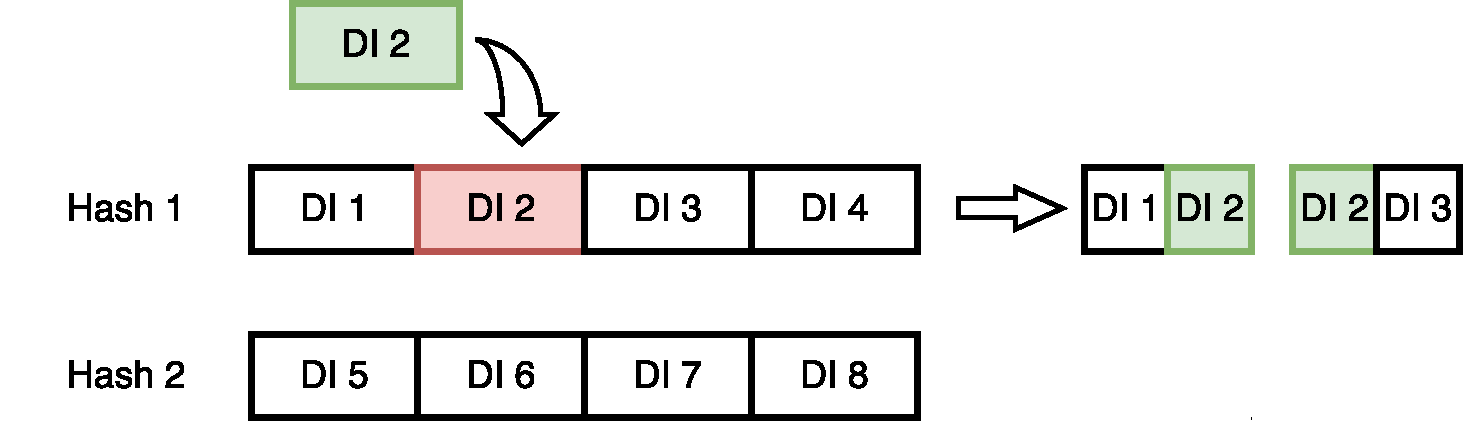
\includegraphics[width=0.48\textwidth]{pics/grouping-invalidation}
  \caption{Invalidation and replaying in grouping}
  \label {grouping-invalidation-figure}
\end{figure}

\subsection{Physical execution and partitioning}

\subsection{Adaptive micro-batching}

\subsubsection{Barrier}

\subsubsection{Minimal time within stream}

\subsection{Fault-tolerance}

\subsection{Guarantees}

\subsubsection{At least once}

\subsubsection{Exactly once}



